\documentclass{article}
\usepackage{graphicx} % Required for inserting images
\usepackage[T2A]{fontenc}
\usepackage{titlesec}
\usepackage[left=25mm, right=15mm, top=20mm, bottom=20mm, footskip=10mm]{geometry}
\usepackage{amsmath}
\usepackage{epigraph}
\usepackage{tikz}
\frenchspacing 
\titleformat{\section}[hang]{\normalsize\bfseries}{\thesection~}{0pt}{}
\titlespacing{\section}{\parindent}{\baselineskip}{\baselineskip}

\titleformat{\subsection}[hang]{\normalsize}{\thesubsection~}{0pt}{}
\titlespacing{\subsection}{\parindent}{0pt}{0pt}
\parindent=1.25cm 

\title{Тема 1. Введение в теорию графов }
\date{}

\begin{document}

\maketitle

\epigraph{Автор конспекта: Родион Лыков}

\epigraph{Чтобы 
удобно и свободно читать данный конспект, убедитесь, что вы знакомы со следующими обозначениями:
\begin{enumerate}
    \item $a \in S$ --- объект $a$ принадлежит множеству $S$
    \item $\forall x$ --- для любого $x$
    \item $\exists x$ --- существует $x$
    \item $(a,b)$ --- пара двух элементов $a,b$
    \item $|S|$ --- размер множества $S$
\end{enumerate}}

\section{Введение}

Граф --- это пара множества вершин $V$ и множества ребер $E$. Обозначают граф $G = (V,E)$. Скорее всего, в своей жизни вы уже встречали графы в том или ином виде. Графы можно встретить в различных областях физики (например, представление электрической цепи в виде графа), в химии (например, представление химического элемента в виде графа). Но больше всего графов встречается в информатике. Итак, давайте приведем пример графа. Элемент множества $E$ --- ребро графа, которое обозначает некую связь между двумя объектами. Объеты --- элементы множества $V$, их называют вершинами графа. Например, вот так можно представить ветку прав, которыми обладают пользователи платформы bacs: администраторы, учителя и ученики: 

\begin{center}
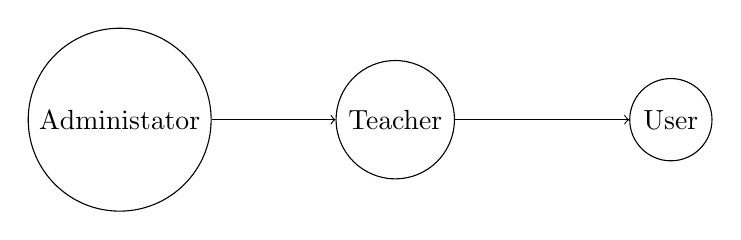
\begin{tikzpicture}[main/.style = {draw, circle},node distance={35mm}] 
\node[main] (1) {$\text{Administator}$}; 
\node[main] (2) [right of=1] {$\text{Teacher}$}; 
\node[main] (3) [right of=2] {$\text{User}$};
\draw[->] (1) -- (2);
\draw[->] (2) -- (3);
\end{tikzpicture} 

Кружочки <<Administator>>, <<Teacher>>, <<User>> называют вершинами (они находятся в множестве $V$), а линии, их соединяющие, называют ребрами
\end{center}

Например, администратор умеет создавать контесты, администратор и учитель могут добавлять новых учеников, в схеме это можно изобразить таким образом:

\begin{center}
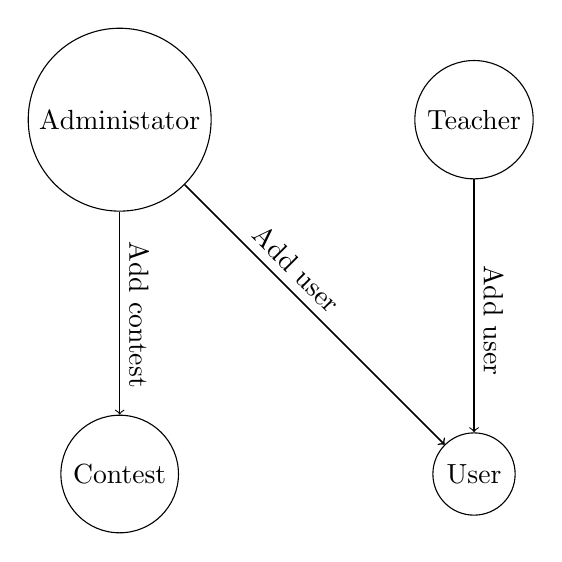
\begin{tikzpicture}[main/.style = {draw, circle},node distance={45mm}] 
\node[main] (1) {$\text{Administator}$}; 
\node[main] (2) [right of=1] {$\text{Teacher}$}; 
\node[main] (4) [below of=1] {$\text{Contest}$};
\node[main] (5) [below of=2] {$\text{User}$};
\draw[->] (1) -- node[above right, sloped, pos=0.1] {Add contest} (4);
\draw[->] (1) -- (5);
\draw[->] (2) -- node[above right, sloped, pos=0.3] {Add user} (5);
\draw[->] (1) -- node[above right, sloped, pos=0.2] {Add user} (5); 
\end{tikzpicture} 

На этой схеме, например, наши ребра означают, к каким функциям есть доступ у определенной группы пользователей. 
\end{center}

Граф обозначает зависимости между парами объектов, например, построим граф где вершины --- это люди, а ребро между двумя людьми обозначает, что люди дружат друг с другом:

\begin{center}
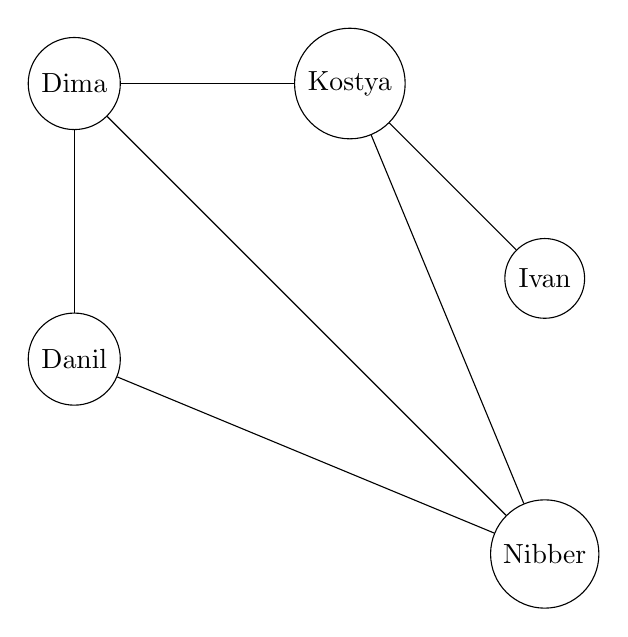
\begin{tikzpicture}[main/.style = {draw, circle},node distance={35mm}] 
\node[main] (1) {$\text{Dima}$}; 
\node[main] (2) [right of=1] {$\text{Kostya}$}; 
\node[main] (3) [below right of=2] {$\text{Ivan}$};
\node[main] (4) [below of=1] {$\text{Danil}$};
\node[main] (5) [below of=3] {$\text{Nibber}$};
\draw (1) -- (4);
\draw (1) -- (5);
\draw (2) -- (5);
\draw (3) -- (2);
\draw (1) -- (2);
\draw (4) -- (5);
\end{tikzpicture}  

Здесь ребра обозначают, дружат ли два объекта друг с другом. 
\end{center}

Думаю, вы заметили, что на первых двух графах ребра были нарисованы со стрелочками, а на последнем --- без. К этому скоро вернемся, пока давайте еще раз проговорим определение графа: граф $G$ есть $(V,E)$. Размер множества $V$ будем обозначать как $n$ (иными словами, $n = |V|$). Размер множества $E$ будем обозначать как $m$ (иными словами, $m = |E|$). Элементом множества $V$ является какой-то объект, в последнем случае это объекты $[\text{Dima},\text{Kostya},
\text{Ivan},\text{Danil},\text{Nibber}]$, ребром является пара двух вершин. Так, в данном графе есть ребра $(\text{Dima}, \text{Kostya}), (\text{Dima}, \text{Danil})$ и другие. Так, ребро есть пара $(a,b)$, где $a,b \in V$. 

Вернемся к стрелочкам. Графы разделяют на ориентированные и неориентированные. В случае неориентированных графов говорят, что ребра являются двусторонними, иными словами ребра $(a,b)$ и $(b,a)$ неразличимы. В случае ориентированных графов у каждого ребра есть свое направление. Таким образом, мы различаем ребра $(a,b)$ и $(b,a)$. Хороший пример таких графов: дороги в городе, где мы разделяем односторонние и двухсторонние дороги. 

Вернемся к вершинам. В примерах для наглядности мы называли их словами, но на практике это неудобно, удобнее пронумеровать вершины, и обращаться к ним по числам. Согласитесь, в программе удобнее будет работать с числами, а не словами. Еще дойдем до графах в программах, пока что продолжим разбираться в базовых терминах графов. 

\section{Основные термины}

\begin{enumerate}
\item Вершина $v$ \textit{инцидентна} ребру $e$, если $v \in e$, иными словами один из концов ребра равен вершине $v$.
\item \textit{Смежными} или же \textit{соседними} называют две вершины, которые соединены ребром. 
\item \textit{Степень} вершины есть количество ребер, инцидентных данной вершине. Будем обозначать степень вершины $v$ как $deg(v)$.
В ориентированном графе разделяют входящую и исходящую степень.
\item \textit{Изолированной} вершиной называется вершина $v$, для которой $deg(v) = 0$.
\item \textit{Висячей} вершиной или \textit{листом} называется вершина $v$, для которой $deg(v) = 1$.
\item \textit{Петлей} называют ребро, которое соединяет вершину с самой собой. 
\item \textit{Смежными} называют два ребра, которые инцидентны одной вершине. 
\item \textit{Путь} в графе есть последовательность смежных ребер. Можно также считать, что путь это 
последовательность смежных вершин. В разных задачах можно определить путь по-разному. 
\item \textit{Путь} называется \textit{простым}, если он проходит через каждую вершину не более одного раза.
\item \textit{Цикл} это такой путь, который заканчивается в той же вершине, что и начинается.
\item \textit{Исток} для ориентированного графа это такая вершина, в которую не направлены ребра.
\item \textit{Сток} для ориентированного графа это такая вершина, из которой не исходит ребер.
\item \textit{Кратное} ребро $(v,u)$ в графе это такое ребро, что существует другое ребро, которое соединяет ту же пару вершин $(v,u)$
(для ориентированного графа порядок важен).
\item \textit{Связным} называется неориентированный граф, для которого между любыми парами вершин существует путь из одной в другую.
\item \textit{Сильно связным} называется ориентированный граф, для которого между любыми парами вершин существует путь из одной в другую.
\item \textit{Компонентой связности} называется такой набор вершин неориентированного графа, что для любой пары вершин из этого набора существует путь из одной в другую.  
\end{enumerate}

Рассмотрим граф, где нет петель и кратных ребер. Сколько максимум ребер может иметь такой граф? 

\section{Виды графов}

Здесь приведем несколько видов графов, с которых начнем знакомство в теории графов. Это не все графы, конечно!

\begin{enumerate}
    \item \textit{Пустым} называется граф без ребер ($m=0$ или же $\forall v \in V : deg(v) = 0$).
    \item \textit{Простым} называется граф без петель и кратных ребер.
    \item \textit{Полным} называется простой граф, в котором максимальное количество ребер. В полном графе $\frac{n(n-1)}{2}$ ребер.
    \item \textit{Разряженным} называют граф, для которого $m = O(n)$.
    \item \textit{Плотным} называют граф, для которого $m = O(n^2)$.
    \item \textit{Деревом} называют связный граф без циклов.  
\end{enumerate}

Остановимся на простых графах поподробнее. Решите следующие задачи на бумаге:

\begin{enumerate}
    \item Сколько может иметь ребер граф на $n$ вершинах?
    \item Докажите, что $m = \frac{1}{2} \sum deg(i)$
    \item Докажите, что в графе существуют, по крайней мере, $2$ вершины, степени
    которых равны.
    \item Докажите, что в графе есть четное количество вершин, у которых степень нечетная. 
    \item Докажите, что если в графе степень каждой вершины не меньше $2$, то в графе есть цикл.
    \item Работает ли это в обратную сторону? (Если в графе есть цикл, то степень каждой вершины не меньше $2$).
    \item Докажите, что если в графе все вершины четные, то в графе нет мостов.
    \item Дайте определение пути в графе между двумя вершинами. 
    \item Дайте определение циклу в графе между двумя вершинами.
    \item Докажите, что если вам дан связный граф на $n$ вершинах и $n-1$ ребром, то в этом графе нет циклов.
\end{enumerate}

А мы приведем решение второй задачи: рассмотрим пустой граф и будем по очереди добавлять в него ребра. Когда мы добавляем очередное ребро, сумма степеней вершин увеличивается на $2$, а количество ребер увеличивается на $1$. Следовательно, если мы разделим сумму степеней вершин, то мы получим количество ребер. 

\section{Представление графов в программе}

Как вы понимаете, рисунки графов мы делаем лишь для более понятного восприятия человеку. Давайте нарисуем два следующих графа:

\begin{center}
\begin{tikzpicture}[main/.style = {draw, circle},node distance={35mm}] 
\node[main] (1) {$1$}; 
\node[main] (2) [right of=1] {$2$}; 
\node[main] (3) [below right of=2] {$3$};
\node[main] (4) [below of=1] {$4$};
\node[main] (5) [right of=2] {$5$};
\draw (1) -- (2);
\draw (2) -- (4);
\draw (1) -- (4);
\draw (2) -- (3);
\end{tikzpicture}  
\end{center}

\begin{center}
\begin{tikzpicture}[main/.style = {draw, circle},node distance={35mm}] 
\node[main] (2) {$2$}; 
\node[main] (4) [right of=2] {$4$}; 
\node[main] (3) [below left of=2] {$3$};
\node[main] (1) [below right of=4] {$1$};
\node[main] (5) [right of=4] {$5$};
\draw (1) -- (2);
\draw (2) -- (4);
\draw (1) -- (4);
\draw (2) -- (3);
\end{tikzpicture}  
\end{center}

Заметьте, что два данных графа полностью одинаковы. Так и программе неважно, как можно нарисовать этот граф, перед нами сейчас стоят следующие цели: как сохранить граф в памяти и как с ним \textbf{удобно} работать и обрабатывать. 
Существуют несколько способов сохранить граф в памяти:

\begin{enumerate}
    \item Список ребер --- перечисление всех ребер в виде одного списка. Самый простой способ, $O(m)$ памяти, однако даже если ребра отсортировать, то быстро найти все ребра, связанные с определенной вершиной будет затруднительно. Подходит в основном для передачи графов и использования их в специфичных алгоритмах. Поэтому редко встречается в решении. 
    В программе список можно реализовать следующим образом:  
    \begin{verbatim}
        vector<pair<int,int>>edges;
        int n,m; // количество вершин и ребер
        cin >> n >> m;
        for(int i = 1; i <= m; i++) {
            int x,y;
            cin >> x >> y;
            edges.push_back({x,y}); // добавляем очередное ребро в список
        }
    \end{verbatim}
    \item Списки смежностей --- $n$ списков, в $i$-м из которых задается список всех вершин смежных $i$-й вершине. Суммарный размер всех списков $2m$, так как каждое ребро добавляет по одному элементу в $2$ списка. $O(n+m)$ памяти, идеально подходит для разреженных графов. Используется практически во всех алгоритмах на разряженных графах. Приведем реализацию:
    \begin{verbatim}
        int n,m; // количество вершин и ребер
        cin >> n >> m;
        vector<vector<int>>e;
        for(int i = 1; i <= m; i++) {
            int x,y;
            cin >> x >> y;
            e[x].push_back(y); // добавляем вершину y в список для x
            e[y].push_back(x); // добавляем вершину x в список для y
        }
    \end{verbatim}
    \item Матрица смежности — матрица $n \times n$, где в ячейке $(x, y)$ хранится количество ребер из вершины $x$ в $y$ (для неориентированных графов симметрична относительно главной диагонали). $O(n^2)$ по памяти, поэтому не подходит для больших разреженных графов, однако хорошо подходит для плотных графов.
    \begin{center}
    Приведем пример матрицы смежности для графа выше
    
    \begin{tabular}{ |c|c|c|c|c| } 
     \hline
     0 & 1 & 0 & 1 & 0  \\ 
     \hline
     1 & 0 & 1 & 1 & 0  \\
     \hline
     0 & 0 & 0 & 1 & 0  \\
     \hline
     1 & 1 & 0 & 0 & 0  \\
     \hline
     0 & 0 & 0 & 0 & 0  \\
     \hline
    \end{tabular}
    \end{center}
    
    \begin{verbatim}
        int n,m; // количество вершин и ребер
        cin >> n >> m;
        vector<vector<int>>mtr(n+1,vector<int>(n+1));
        for(int i = 1; i <= m; i++) {
            int x,y;
            cin >> x >> y;
            mtr[x][y] += 1;
            mtr[y][x] += 1;
        }
    \end{verbatim}
    
    \item Матрица инцидентности --- матрица $n \times m$ где в ячейке $(x, y)$ хранится $1$ если вершина $x$ инцидентна ребру $y$, а иначе $0$. Для ориентированных графов также разделяют $1$ и $-1$: $-1$ для вершины, в которой начинается ребро, а $-1$ --- для вершины, в которой оно заканчивается. $O(n \cdot m)$ памяти, очень громоздкая и на практике практически не используется.
    
    \begin{center}
        Приведем пример матрицы инцидентности для графа выше:
        
         \begin{tabular}{ |c|c|c|c| } 
         \hline
         1 & 1 & 0 & 0  \\ 
         \hline
         1 & 0 & 1 & 1   \\
         \hline
         0 & 0 & 0 & 1   \\
         \hline
         0 & 1 & 1 & 0  \\
         \hline
         0 & 0 & 0 & 0   \\
         \hline
        \end{tabular}
    \end{center}
        \begin{verbatim}
            int n,m; // количество вершин и ребер
            cin >> n >> m;
            vector<vector<int>>mtr(n+1,vector<int>(m+1));
            for(int i = 1; i <= m; i++) {
                int x,y;
                cin >> x >> y;
                mtr[x][i] = 1;
                mtr[y][i] = 1;
            }
        \end{verbatim}

\end{enumerate}

Покажем решение задачи <<Степень+еориентированный>>. 
В этой задаче нам нужно по матрице смежности определить количество ребер в графе и степень каждой вершины.
\begin{verbatim}
#include <bits/stdc++.h>
using namespace std;
int main() {
    int n;
    cin >> n;
    vector<vector<int>>mtr(n+1,vector<int>(n+1));
    int sum_deg = 0;
    vector<int>ans(n+1);
    for(int i = 1; i <= n; i++) {
        for(int j = 1; j <= n; j++) {
            cin >> mtr[i][j];
            ans[i] += mtr[i][j];
        }
        sum_deg += ans[i];
    }
    cout << sum_deg / 2 << endl;
    cout << ans[1];
    for(int i = 2; i <= n; i++) {
        cout << " " << ans[i];
    }
}
        \end{verbatim}

\end{document}
